\documentclass[12pt,a4paper]{article}
\usepackage[utf8]{inputenc}
\usepackage[T2A]{fontenc}
\usepackage[russian]{babel}
\usepackage{graphicx}
\usepackage{booktabs}
\usepackage{longtable}
\usepackage{geometry}
\usepackage{float}
\geometry{top=2cm, left=2cm, right=2cm, bottom=2cm}
\usepackage{paracol}
\usepackage{src/title}
\usepackage{hyperref}
\usepackage{listings}
\usepackage{xcolor}

\title{Лабораторная работа 4. Метод k-ближайших соседей}
\author{Ануфриев А.С. 465029}
\supervisor{Болдырева Е. А.}
\date{07.11.2026}

\abstract{
На исходных данных о вине выполнена предобработка, получена описательная статистика и 3D-визуализация признаков. Реализован метод k-ближайших соседей собственным кодом на Python (NumPy, Pandas) без готовых библиотек классификации. Построены две модели k-NN (случайный и фиксированный наборы признаков), проведена оценка на тестовой выборке при различных k с построением матриц ошибок.
}
\keywords{k-ближайших соседей, классификация, датасет о вине, NumPy, матрица ошибок}

\begin{document}
\maketitle

\section{Цели и задачи}
Цель работы --- исследование и применение метода k-ближайших соседей (k-NN) для классификации winetime-датасета о вине. Основные задачи:
\begin{enumerate}
\item получить и визуализировать описательную статистику по датасету (количество, среднее, стандартное отклонение, минимум, максимум, квантили);
\item выполнить предобработку данных: обработку отсутствующих значений, кодирование категориальных признаков, масштабирование;
\item построить 3D-визуализацию признаков;
\item реализовать метод k-ближайших соседей собственным кодом без использования готовых библиотек классификации (только NumPy и Pandas);
\item построить две модели k-NN: со случайным и с фиксированным наборами признаков;
\item оценить каждую модель на тестовой выборке при различных k и построить матрицы ошибок.
\end{enumerate}

\section{Исходные данные}
Исходный датасет содержит 178 записей о вине. Признаков: 13 числовых (Alcohol, Malic Acid, Ash, Alcalinity of ash, Magnesium, Total phenols, Flavanoids, Nonflavanoid phenols, Proanthocyanins, Color intensity, Hue, OD280/OD315 of diluted wines, Proline). Целевая переменная --- Wine (три класса: 1, 2, 3). Пропущенных значений и категориальных признаков в данных не обнаружено.

\section{Теоретические сведения}
Метод k-ближайших соседей относит объект к классу, наиболее часто встречающемуся среди k ближайших соседей в пространстве признаков. Расстояние между объектами вычисляется по правилу Евклида:
\begin{equation}
d(\mathbf{x}_i, \mathbf{x}_j) = \sqrt{\sum_{p=1}^{P} (x_{ip} - x_{jp})^2}.
\end{equation}
Класс объекта определяется majoritaire голосованием среди k ближайших обучающих примеров. Качество классификации оценивается долей верных предсказаний (accuracy) и матрицей ошибок.

\section{Ход работы}
\subsection{Предобработка данных}
В данных отсутствуют пропущенные значения и категориальные признаки. Все 13 числовых признаков подвергнуты стандартизации (вычет среднего, деление на стандартное отклонение). Данные разделены на обучающую (142 записи, 80\%) и тестовую (36 записей, 20\%) выборки с фиксированным зерном случайности для воспроизводимости.

\subsection{Реализация метода k-NN}
Метод k-ближайших соседей реализован собственным кодом на Python с использованием NumPy: парные евклидовые расстояния вычисляются матрично, за ним folgt сортировка и выбор k ближайших соседей, класс определяется голосованием. Готовые средства классификации не использовались.

\subsection{Модели}
Построены две модели (зерно случайности random\_state = 42 для воспроизводимости):
\begin{itemize}
\item Модель 1 --- признаки отбираются случайно (5 из 13: Alcohol, Color intensity, OD280/OD315 of diluted wines, Proanthocyanins, Total phenols);
\item Модель 2 --- фиксированный набор признаков, выбранный заранее (Alcohol, Malic Acid, Ash, Alcalinity of ash, Magnesium, Total phenols).
\end{itemize}
Для каждой модели оценка проведена при k = 3, 5, 10, 15.

\section{Результаты}
\subsection{Описательная статистика}
Получена описательная статистика по всем признакам (таблица~\ref{tab:stats}), построены гистограммы распределения признаков (рисунок~\ref{fig:hist}) и средние значения признаков (рисунок~\ref{fig:means}). Для наглядности выполнена 3D-визуализация первых трёх признаков, окрашенная по классам (рисунок~\ref{fig:3d}).

\begin{table}[H]
\centering
\caption{Описательная статистика по датасету.}
\label{tab:stats}
\small
\begin{tabular}{lrrrrrrrr}
\toprule
Признак & count & mean & std & min & q25 & q50 & q75 & max \\
\midrule
Alcohol & 178 & 13.00 & 0.81 & 11.03 & 12.36 & 13.05 & 13.68 & 14.83 \\
Malic Acid & 178 & 2.34 & 1.12 & 0.74 & 1.60 & 1.87 & 3.08 & 5.80 \\
Ash & 178 & 2.37 & 0.27 & 1.36 & 2.21 & 2.36 & 2.56 & 3.23 \\
Alcalinity of ash & 178 & 19.50 & 3.34 & 10.60 & 17.20 & 19.50 & 21.50 & 30.00 \\
Magnesium & 178 & 99.74 & 14.28 & 70.00 & 88.00 & 98.00 & 107.00 & 162.00 \\
Total phenols & 178 & 2.30 & 0.63 & 0.98 & 1.74 & 2.36 & 2.80 & 3.88 \\
Flavanoids & 178 & 2.03 & 1.00 & 0.34 & 1.21 & 2.14 & 2.88 & 5.08 \\
\bottomrule
\end{tabular}
\end{table}

\begin{table}[H]
\centering
\caption{Описательная статистика по датасету (продолжение).}
\label{tab:stats2}
\small
\begin{tabular}{lrrrrrrrr}
\toprule
Признак & count & mean & std & min & q25 & q50 & q75 & max \\
\midrule
Nonflavanoid phenols & 178 & 0.36 & 0.12 & 0.13 & 0.27 & 0.34 & 0.44 & 0.66 \\
Proanthocyanins & 178 & 1.59 & 0.57 & 0.41 & 1.25 & 1.56 & 1.95 & 3.58 \\
Color intensity & 178 & 5.06 & 2.32 & 1.28 & 3.22 & 4.69 & 6.20 & 13.00 \\
Hue & 178 & 0.96 & 0.23 & 0.48 & 0.78 & 0.97 & 1.12 & 1.71 \\
OD280/OD315 of diluted wines & 178 & 2.61 & 0.71 & 1.27 & 1.94 & 2.78 & 3.17 & 4.00 \\
Proline & 178 & 746.89 & 314.91 & 278.00 & 500.50 & 673.50 & 985.00 & 1680.00 \\
\bottomrule
\end{tabular}
\end{table}

\begin{figure}[H]
\centering
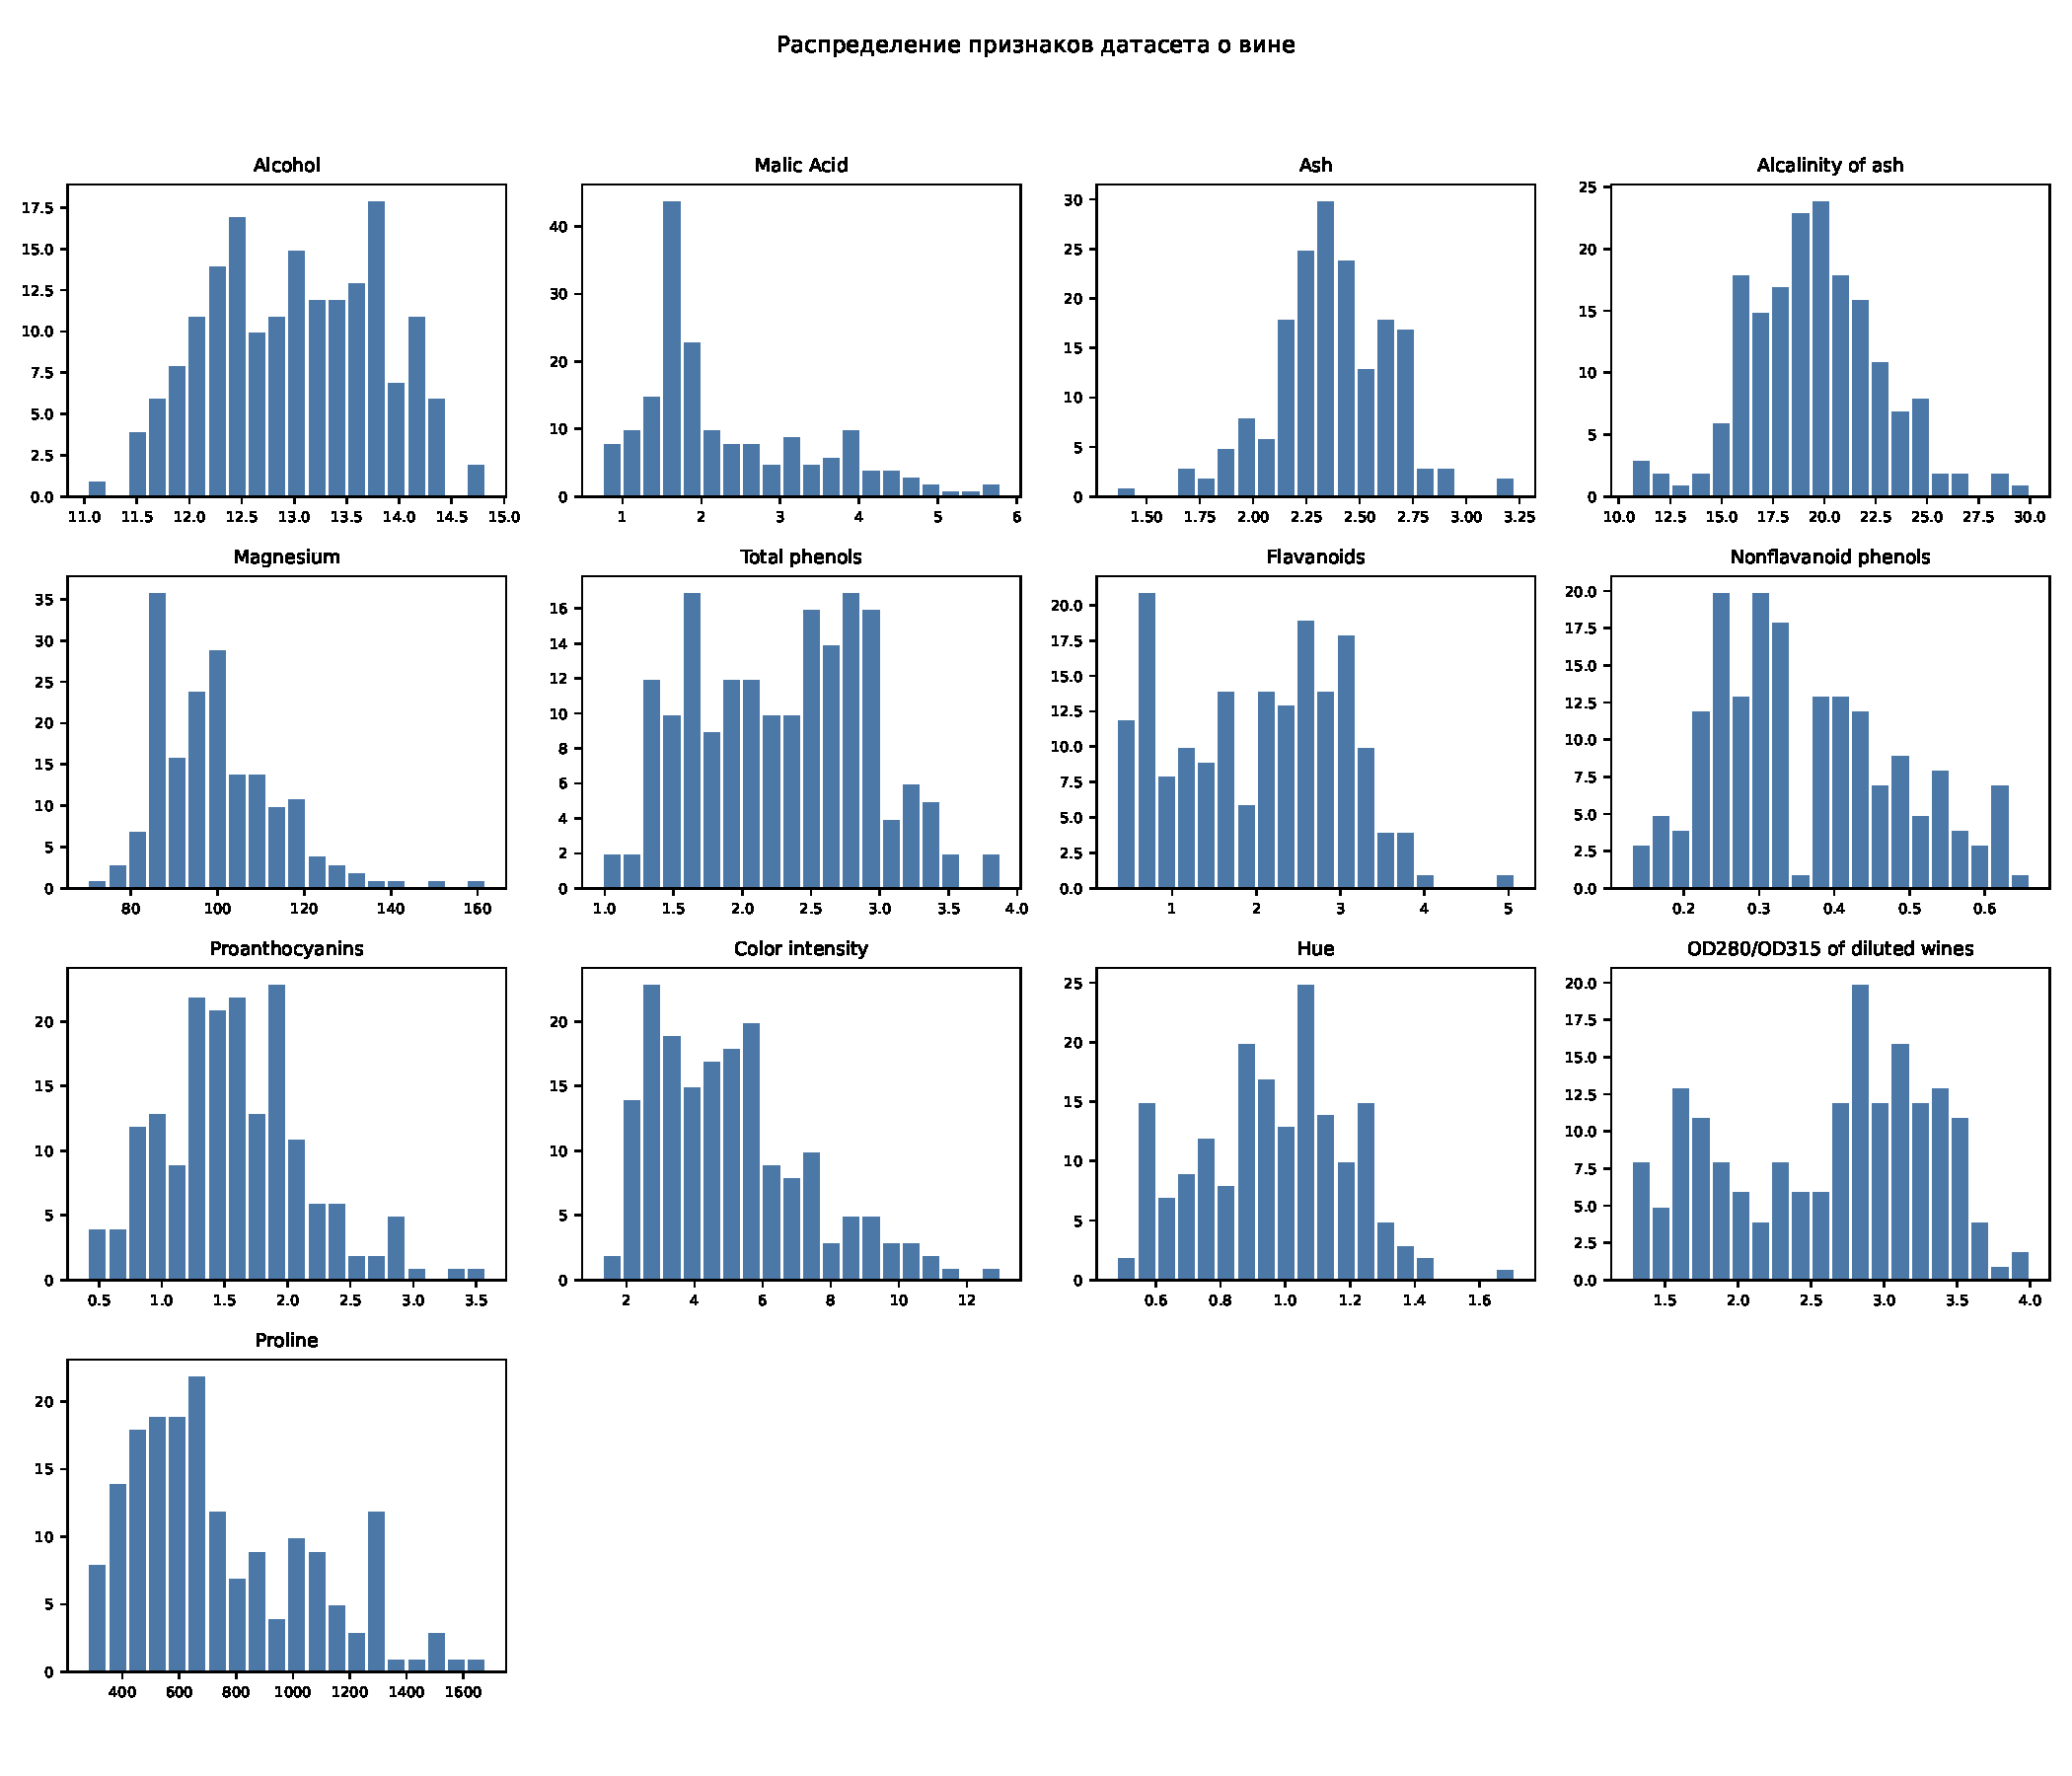
\includegraphics[width=0.9\linewidth]{../graphics/feature_histograms.pdf}
\caption{Распределение признаков датасета о вине.}
\label{fig:hist}
\end{figure}

\begin{figure}[H]
\centering
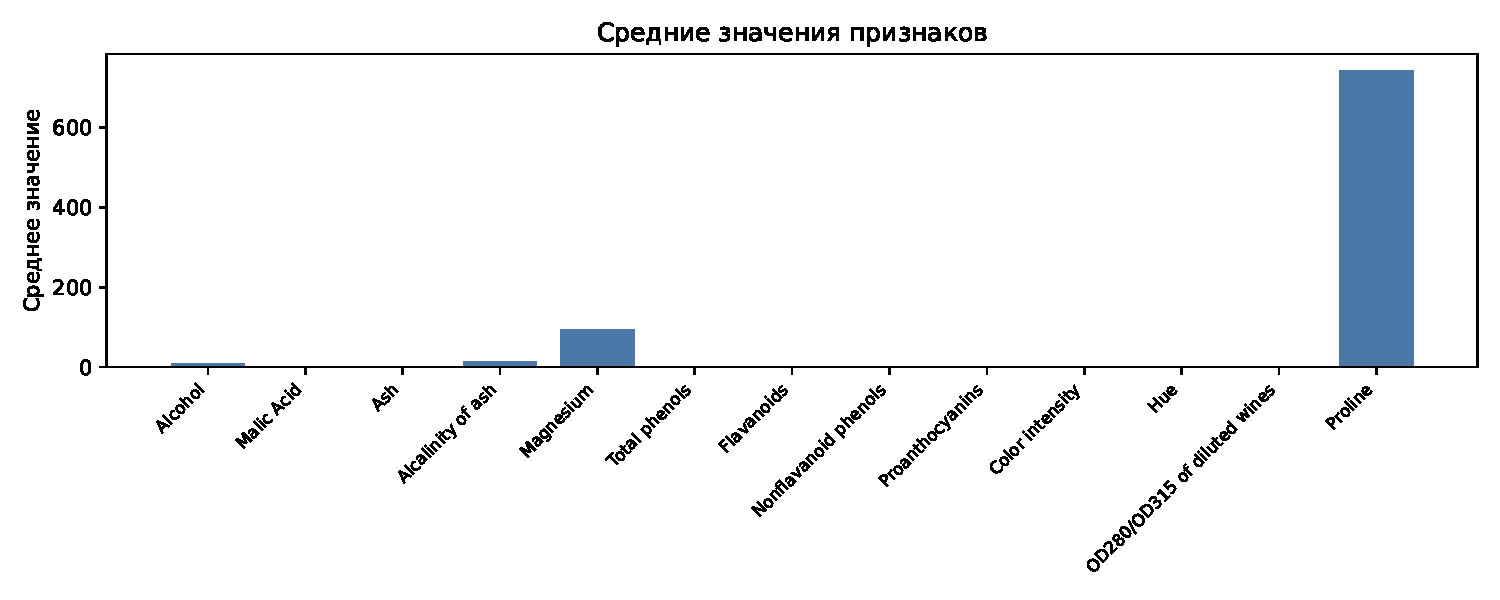
\includegraphics[width=0.7\linewidth]{../graphics/feature_means.pdf}
\caption{Средние значения признаков.}
\label{fig:means}
\end{figure}

\begin{figure}[H]
\centering
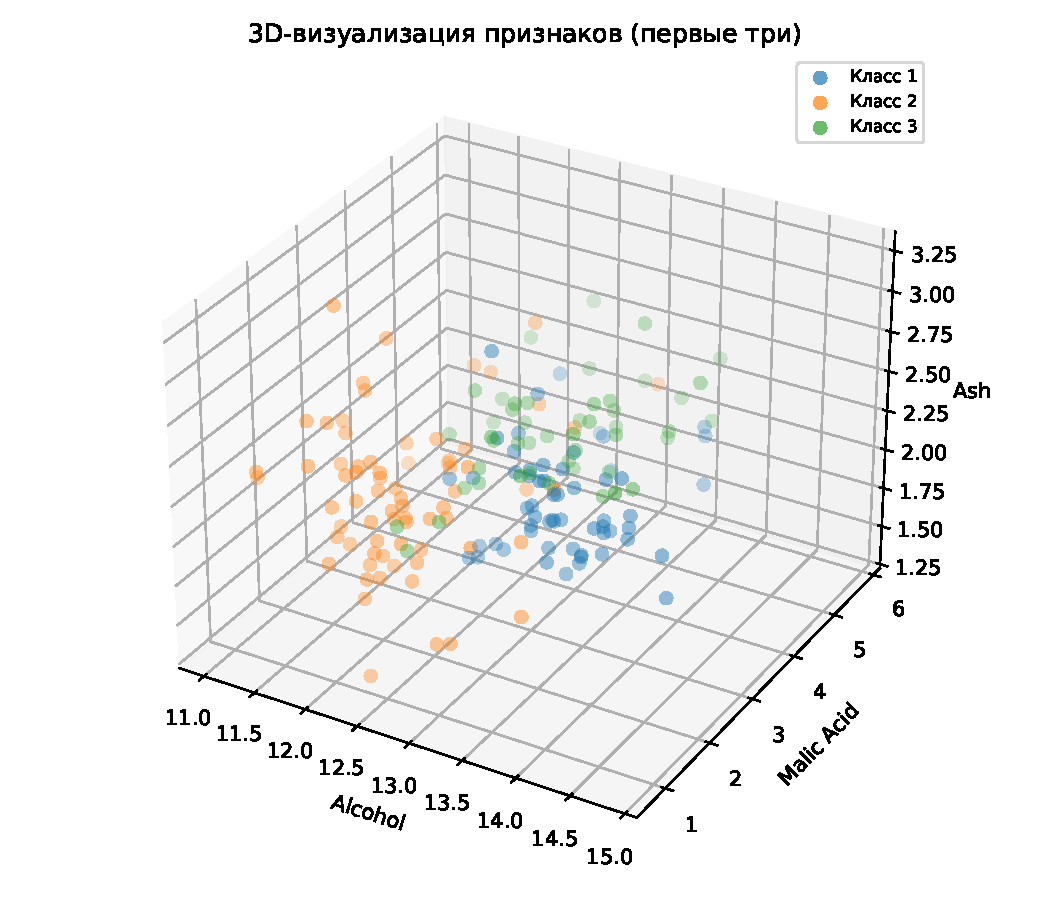
\includegraphics[width=0.7\linewidth]{../graphics/visualization_3d.pdf}
\caption{3D-визуализация признаков (первые три), окрашенная по классам.}
\label{fig:3d}
\end{figure}

\subsection{Качество классификации}
Точность классификации (accuracy) на тестовой выборке при различных k приведена в таблице~\ref{tab:metrics}.

\begin{table}[H]
\centering
\caption{Точность k-NN на тестовой выборке.}
\label{tab:metrics}
\small
\begin{tabular}{llcccc}
\toprule
Модель & Признаки & k=3 & k=5 & k=10 & k=15 \\
\midrule
Модель 1 & случайные (5 признаков) & 0.9444 & 0.9444 & 0.9167 & 0.9167 \\
Модель 2 & фиксированные (6 признаков) & 0.8889 & 0.8889 & 0.9444 & 0.9444 \\
\bottomrule
\end{tabular}
\end{table}

\subsection{Матрицы ошибок}
Матрицы ошибок для всех пар модель $\times$ k на тестовой выборке (строки --- истинные классы 1, 2, 3; столбцы --- предсказанные классы 1, 2, 3; в каждой ячейке элементы строки матрицы перечислены через ``; ''):

\begin{table}[H]
\centering
\caption{Матрицы ошибок k-NN на тестовой выборке.}
\label{tab:allcm}
\small
\begin{tabular}{llclll}
\toprule
Модель & k & Точность & Матрица, строка 1 & строка 2 & строка 3 \\
\midrule
Модель 1 & 3 & 0.9444 & 14; 0; 0 & 1; 12; 1 & 0; 0; 8 \\
Модель 1 & 5 & 0.9444 & 14; 0; 0 & 1; 12; 1 & 0; 0; 8 \\
Модель 1 & 10 & 0.9167 & 14; 0; 0 & 1; 11; 2 & 0; 0; 8 \\
Модель 1 & 15 & 0.9167 & 14; 0; 0 & 1; 11; 2 & 0; 0; 8 \\
Модель 2 & 3 & 0.8889 & 12; 0; 2 & 1; 12; 1 & 0; 0; 8 \\
Модель 2 & 5 & 0.8889 & 13; 0; 1 & 0; 12; 2 & 0; 1; 7 \\
Модель 2 & 10 & 0.9444 & 13; 0; 1 & 0; 14; 0 & 0; 1; 7 \\
Модель 2 & 15 & 0.9444 & 13; 0; 1 & 1; 13; 0 & 0; 0; 8 \\
\bottomrule
\end{tabular}
\end{table}

Матрицы ошибок для каждой модели при k, дающем наилучшую точность (таблица~\ref{tab:cm1} и таблица~\ref{tab:cm2}).

\begin{table}[H]
\centering
\caption{Матрица ошибок, Модель 1, k=5.}
\label{tab:cm1}
\small
\begin{tabular}{lccc}
\toprule
 & \multicolumn{3}{c}{Предсказанный класс} \\
Истинный класс & 1 & 2 & 3 \\
\midrule
1 & 14 & 0 & 0 \\
2 & 1 & 12 & 1 \\
3 & 0 & 0 & 8 \\
\bottomrule
\end{tabular}
\end{table}

\begin{table}[H]
\centering
\caption{Матрица ошибок, Модель 2, k=10.}
\label{tab:cm2}
\small
\begin{tabular}{lccc}
\toprule
 & \multicolumn{3}{c}{Предсказанный класс} \\
Истинный класс & 1 & 2 & 3 \\
\midrule
1 & 13 & 0 & 1 \\
2 & 0 & 14 & 0 \\
3 & 0 & 1 & 7 \\
\bottomrule
\end{tabular}
\end{table}

\begin{figure}[H]
\centering
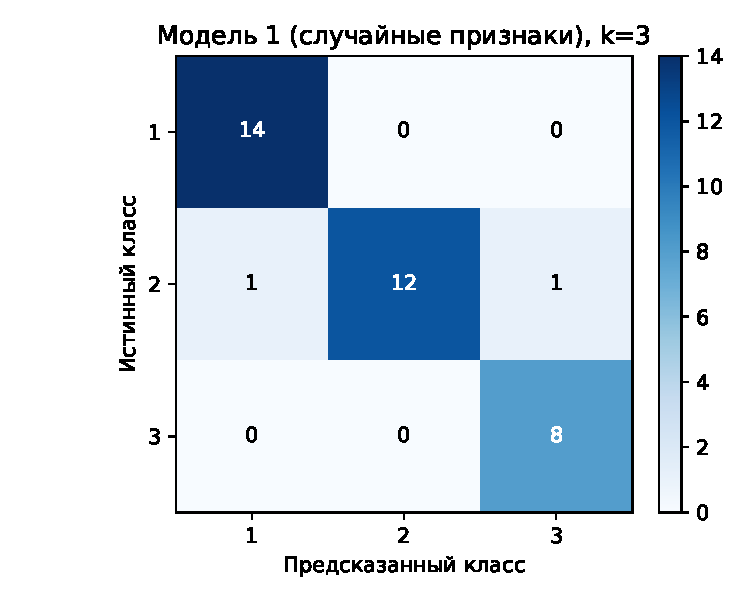
\includegraphics[width=0.45\linewidth]{../graphics/confusion_model1.pdf}
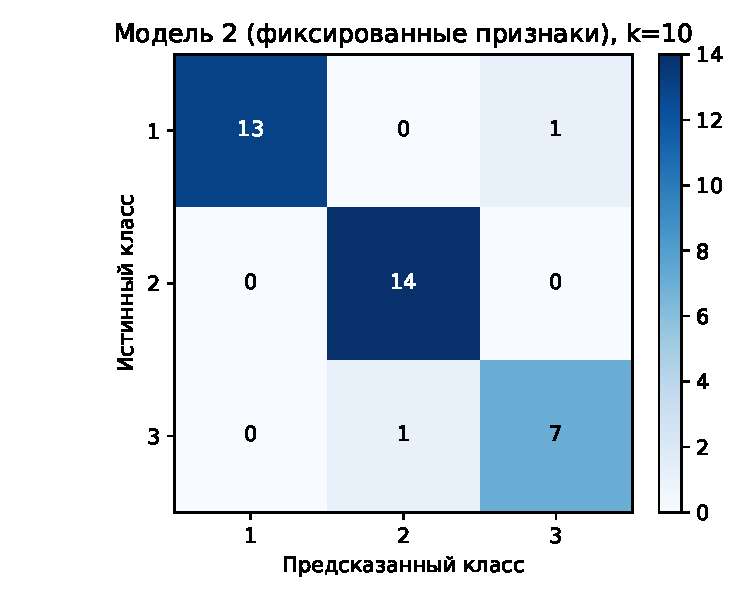
\includegraphics[width=0.45\linewidth]{../graphics/confusion_model2.pdf}
\caption{Матрицы ошибок: Модель 1 (слева, k=5) и Модель 2 (справа, k=10).}
\label{fig:cm}
\end{figure}

\section{Выводы}
Реализован метод k-ближайших соседей без готовых библиотек классификации. Обе модели обеспечивают высокую точность на тестовой выборке (до 0.9444). Модель 1 с случайным набором признаков стабильна при k=3 и k=5 (0.9444), Модель 2 с фиксированным набором достигает наилучшего результата при k=10 и k=15 (0.9444). Матрицы ошибок показывают, что основные ошибки приходятся на путаницу между классами 2 и 3.

\section{Приложение}
Полный фрагмент реализации метода k-ближайших соседей (NumPy). X и y --- признаки и метки классов после загрузки и предобработки датасета (стандартизация: вычет среднего, деление на стандартное отклонение); random\_state = 42.
\begin{lstlisting}[language=Python, basicstyle=\footnotesize\ttfamily]
import numpy as np

rng = np.random.RandomState(42)
n = X.shape[0]
idx = rng.permutation(n)
n_test = int(round(0.2 * n))
train_idx, test_idx = idx[n_test:], idx[:n_test]
X_tr, X_te = X[train_idx], X[test_idx]
y_tr, y_te = y[train_idx], y[test_idx]

class KNN:
    def __init__(self, k=3):
        self.k = k
    def fit(self, X, y):
        self.X = np.asarray(X, float); self.y = np.asarray(y)
    def predict(self, X):
        X = np.asarray(X, float)
        a2 = np.sum(X**2, axis=1, keepdims=True)
        b2 = np.sum(self.X**2, axis=1, keepdims=True).T
        ab = X @ self.X.T
        d = np.sqrt(np.maximum(a2 + b2 - 2*ab, 0.0))
        nb = np.argsort(d, axis=1)[:, :self.k]
        return np.array([np.bincount(self.y[nb[i]].astype(int)).argmax()
                         for i in range(X.shape[0])])

def accuracy(y_true, y_pred):
    return float(np.mean(y_true == y_pred))

for k in (3, 5, 10, 15):
    clf = KNN(k=k)
    clf.fit(X_tr, y_tr)
    print(k, accuracy(y_te, clf.predict(X_te)))
\end{lstlisting}

\section{Литература}
\begin{enumerate}
\item Лабораторное задание №4. Метод k-ближайших соседей.
\item Датасет о вине WineDataset.csv (исходные данные).
\item NumPy --- библиотека для научных вычислений на языке Python.
\item Pandas --- библиотека для анализа и обработки данных.
\end{enumerate}

\end{document}
